\begin{figure}[H]
\centering
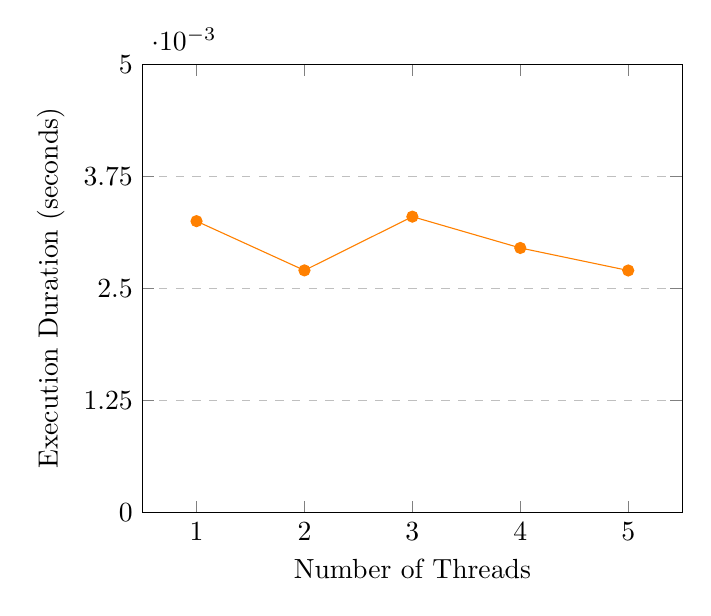
\begin{tikzpicture}
\begin{axis}[
    xlabel={Number of Threads},
    ylabel={Execution Duration (seconds)},
    xmin=0.5, xmax=5.5,
    ymin=0, ymax=0.005,
    xtick={1, 2, 3, 4, 5},
    ytick={0, 0.00125, 0.0025, 0.00375, 0.005},
    ymajorgrids=true,
    grid style=dashed,
]
\addplot[
    color=orange,
    mark=*,
    ]
    coordinates {
    (1,0.003249520) (2,0.002700380) (3,0.003299843) (4,0.002950533) (5,0.002699282)
    };

\end{axis}
\end{tikzpicture}
\caption{Execution Duration vs. Number of Threads for Hepta}
\label{fig:hepta}
\end{figure}